% =====================================================================
%  Final report -- SunSand IoT Monitor (Microprocessor course project)
%  Compile: xelatex report.tex   (run twice for the TOC + TikZ)
% =====================================================================
\documentclass[11pt,a4paper]{article}

\usepackage[margin=2.2cm,top=2.4cm,bottom=2.6cm]{geometry}
\usepackage{fontspec}
\usepackage{xcolor}
\usepackage{booktabs}
\usepackage{array}
\usepackage{longtable}
\usepackage{enumitem}
\usepackage{titlesec}
\usepackage{fancyhdr}
\usepackage{parskip}
\usepackage[hidelinks]{hyperref}
\usepackage{listings}
\usepackage{tikz}
\usetikzlibrary{automata, positioning, arrows.meta, shapes.geometric, calc}

\definecolor{accent}{HTML}{1F4E78}
\definecolor{mute}{HTML}{555555}
\definecolor{soft}{HTML}{F0F4FA}
\definecolor{okbg}{HTML}{E2EFDA}
\definecolor{okfg}{HTML}{2E7D32}

\titleformat{\section}{\Large\bfseries\color{accent}}{\thesection.}{0.6em}{}
\titleformat{\subsection}{\large\bfseries\color{accent}}{\thesubsection}{0.5em}{}

\pagestyle{fancy}\fancyhf{}
\fancyhead[L]{\small\color{mute}SunSand IoT Monitor --- Final Report}
\fancyhead[R]{\small\color{mute}\thepage}
\renewcommand{\headrulewidth}{0pt}

\newcommand{\fillin}[1]{{\color{okfg}\textbf{[FILL IN: #1]}}}
\newcommand{\note}[1]{\par\medskip\noindent\colorbox{soft}{\parbox{\dimexpr\linewidth-2\fboxsep}{\small #1}}\medskip\par}
\newcommand{\ok}[1]{\par\medskip\noindent\colorbox{okbg}{\parbox{\dimexpr\linewidth-2\fboxsep}{\small\color{okfg}#1}}\medskip\par}

\setlength{\parindent}{0pt}
\setlist{topsep=2pt,itemsep=2pt}
\lstset{basicstyle=\ttfamily\footnotesize,frame=single,
  rulecolor=\color{mute!40},backgroundcolor=\color{soft},
  breaklines=true,columns=fullflexible,keepspaces=true,
  showstringspaces=false,language=C}

\title{\textbf{SunSand IoT Monitor}\\[0.3em]
\large A two-node LoRa wireless sensor system with a live dashboard\\[0.4em]
\normalsize Microprocessor Course --- Project Report}
\author{\fillin{team member names + IDs}}
\date{2026-05-17}

\begin{document}
\maketitle
\thispagestyle{empty}
\begin{center}\small\color{mute}
Project idea \#4 --- IoT Environmental Monitor (extended to two nodes + a LoRa gateway).
\end{center}
\vspace{0.4em}
\tableofcontents
\newpage

% ---------------------------------------------------------------------
\section{Objective}
% ---------------------------------------------------------------------

Build a wireless environmental \& security monitoring system around the
ESP32 microcontroller. Two battery-class sensor nodes each read a small
set of sensors and transmit the readings over a 433~MHz LoRa radio link
to a third ESP32 acting as a gateway. The gateway has no sensors; it
relays every received packet to a laptop over USB serial, where a
dashboard displays the live data.

This is project idea \#4 from the brief (IoT Environmental Monitor),
deliberately extended from a single board to a \emph{three-board wireless
network} so it exercises a broader range of microprocessor concepts:
digital sensor protocols, the I\textsuperscript{2}C bus, GPIO interrupts,
SPI driving an RF transceiver, UART to a host, and an explicit
finite-state-machine firmware architecture on each board.

% ---------------------------------------------------------------------
\section{System overview}
% ---------------------------------------------------------------------

\begin{center}
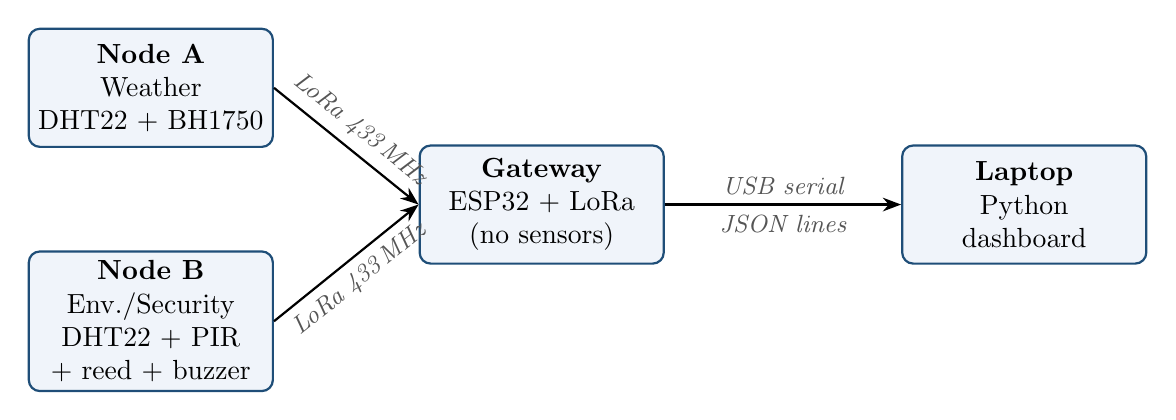
\begin{tikzpicture}[
  box/.style={draw=accent,thick,rounded corners,fill=soft,
              align=center,minimum height=1.5cm,minimum width=3.1cm},
  lbl/.style={font=\small\itshape,color=mute},
  >=Stealth]
  \node[box] (A) {\textbf{Node A}\\Weather\\DHT22 + BH1750};
  \node[box, below=1.3cm of A] (B) {\textbf{Node B}\\Env./Security\\DHT22 + PIR\\+ reed + buzzer};
  \node[box, right=3.4cm of $(A)!0.5!(B)$] (G) {\textbf{Gateway}\\ESP32 + LoRa\\(no sensors)};
  \node[box, right=3.0cm of G] (L) {\textbf{Laptop}\\Python\\dashboard};
  \draw[->,thick] (A.east) -- node[lbl,above,sloped]{LoRa 433\,MHz} (G.west);
  \draw[->,thick] (B.east) -- node[lbl,below,sloped]{LoRa 433\,MHz} (G.west);
  \draw[->,thick] (G.east) -- node[lbl,above]{USB serial} node[lbl,below]{JSON lines} (L.west);
\end{tikzpicture}
\end{center}

The two sensor nodes are transmit-only; the gateway is receive-only on
the radio side and transmit-only on the USB side. There is no return
path in this version --- a deliberate scope choice that keeps the demo
rock-solid (no WiFi, no broker, no network configuration in the exam
room). The architecture is identical to a production wireless-sensor
network; only the gateway's output stage (USB serial here) would change
to WiFi/MQTT in a deployed system.

% ---------------------------------------------------------------------
\section{Hardware design}
% ---------------------------------------------------------------------

\subsection{Sensors and components}

\begin{longtable}{@{}llp{7.4cm}@{}}
\toprule
\textbf{Component} & \textbf{Interface} & \textbf{Role}\\
\midrule\endhead
ESP32-WROOM-32 DevKit ($\times$3) & ---       & Microcontroller for each node + gateway\\
LoRa Ra-01 (SX1278) ($\times$3)   & SPI       & 433~MHz radio transceiver\\
DHT22 / AM2302 ($\times$2)        & 1-wire digital & Temperature + humidity (node A and B)\\
BH1750 ($\times$1)                & I\textsuperscript{2}C & Ambient light, lux (node A)\\
HC-SR501 PIR ($\times$1)          & GPIO digital & Motion detection (node B)\\
Reed switch + magnet ($\times$1)  & GPIO digital & Door open/closed (node B)\\
Active buzzer ($\times$1)         & GPIO digital & Audible alarm (node B, bonus)\\
\bottomrule
\end{longtable}

\subsection{Pin assignments}

The LoRa SPI bus is fixed by the ESP32's VSPI peripheral and is the same
on all three boards:

\begin{center}\begin{tabular}{@{}llll@{}}
\toprule
SCK & MISO & MOSI & NSS / RST / DIO0\\
\midrule
GPIO18 & GPIO19 & GPIO23 & GPIO5 / GPIO27 / GPIO26\\
\bottomrule
\end{tabular}\end{center}

\begin{center}\begin{tabular}{@{}lll@{}}
\toprule
\textbf{Board} & \textbf{Sensor / actuator} & \textbf{ESP32 pin}\\
\midrule
Node A & DHT22 DATA          & GPIO4 \\
Node A & BH1750 SDA / SCL    & GPIO21 / GPIO22 (I\textsuperscript{2}C) \\
Node B & DHT22 DATA          & GPIO4 \\
Node B & HC-SR501 OUT        & GPIO34 (input) \\
Node B & Reed switch         & GPIO32 (\texttt{INPUT\_PULLUP}, other leg to GND) \\
Node B & Buzzer              & GPIO25 (output) \\
Gateway & (none)             & --- \\
\bottomrule
\end{tabular}\end{center}

\note{The Ra-01 is a 3.3~V part --- it is powered from the ESP32's 3V3
pin, never 5~V. A 100~nF ceramic capacitor sits across its VCC--GND
pins for decoupling. The reed switch uses the ESP32's internal pull-up
so no external resistor is required.}

\subsection{Circuit schematic}

\begin{center}
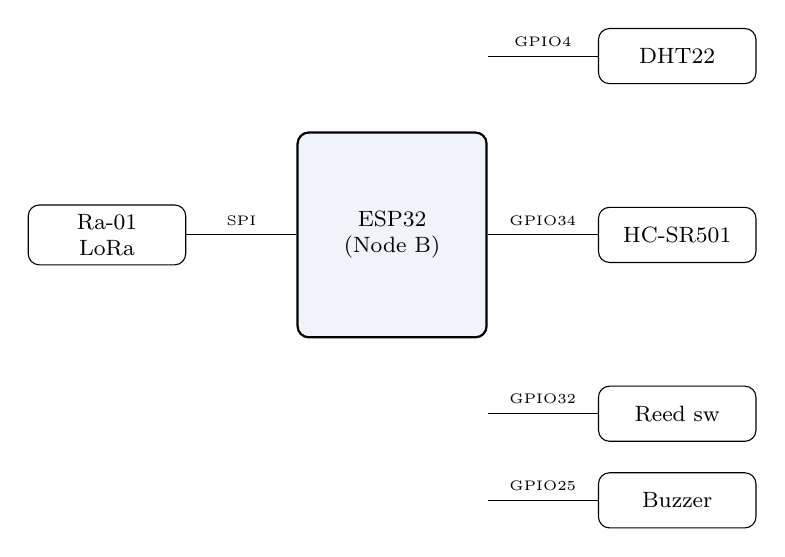
\begin{tikzpicture}[font=\footnotesize,
  chip/.style={draw,thick,rounded corners,fill=soft,minimum width=2.4cm,
               minimum height=2.6cm,align=center},
  per/.style={draw,rounded corners,fill=white,minimum width=2.0cm,
              minimum height=0.7cm,align=center}]
  % Node B (most complete) shown as the representative schematic
  \node[chip] (esp) {ESP32\\(Node B)};
  \node[per, above right=0.6cm and 1.4cm of esp] (dht) {DHT22};
  \node[per, right=1.4cm of esp] (pir) {HC-SR501};
  \node[per, below right=0.6cm and 1.4cm of esp] (reed) {Reed sw};
  \node[per, below right=1.7cm and 1.4cm of esp] (buz) {Buzzer};
  \node[per, left=1.4cm of esp] (lora) {Ra-01\\LoRa};
  \draw (esp.east|-dht) -- (dht.west) node[midway,above,font=\tiny]{GPIO4};
  \draw (esp.east|-pir) -- (pir.west) node[midway,above,font=\tiny]{GPIO34};
  \draw (esp.east|-reed) -- (reed.west) node[midway,above,font=\tiny]{GPIO32};
  \draw (esp.east|-buz) -- (buz.west) node[midway,above,font=\tiny]{GPIO25};
  \draw (esp.west) -- (lora.east) node[midway,above,font=\tiny]{SPI};
\end{tikzpicture}\\[4pt]
{\small\itshape Representative schematic (Node B). Node A replaces
PIR/reed/buzzer with a BH1750 on the I\textsuperscript{2}C bus; the
gateway has only the ESP32 + Ra-01.}
\end{center}

% ---------------------------------------------------------------------
\section{Software design}
% ---------------------------------------------------------------------

Every board runs a single, explicit finite state machine in its Arduino
\texttt{loop()}: an \texttt{enum} of states and a \texttt{switch} that
executes one state per iteration and decides the next state. This makes
the firmware behaviour directly traceable to the diagrams below --- each
\texttt{case} in the code is one bubble in the diagram.

\subsection{Node A --- weather (state machine)}

\begin{center}
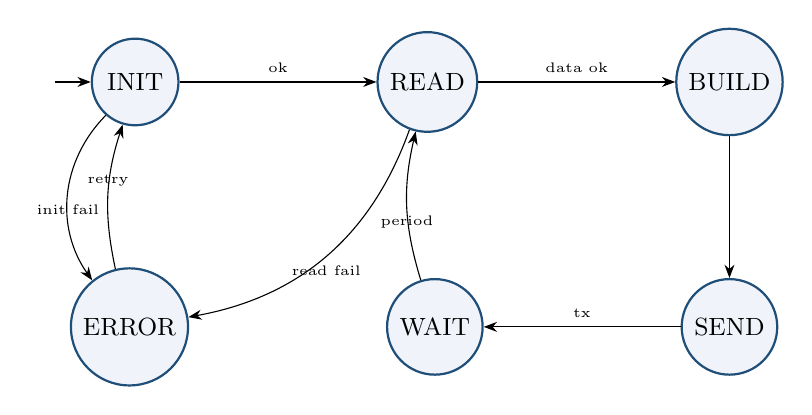
\begin{tikzpicture}[->,>=Stealth,node distance=2.5cm,
  every state/.style={draw=accent,thick,fill=soft,minimum size=1.1cm,
                       font=\small}]
  \node[state,initial,initial text=] (I) {INIT};
  \node[state, right=of I] (R) {READ};
  \node[state, right=of R] (Bu) {BUILD};
  \node[state, below=1.8cm of Bu] (S) {SEND};
  \node[state, left=of S] (W) {WAIT};
  \node[state, left=of W] (E) {ERROR};
  \path (I) edge node[above,font=\tiny]{ok} (R)
        (R) edge node[above,font=\tiny]{data ok} (Bu)
        (Bu) edge (S)
        (S) edge node[above,font=\tiny]{tx} (W)
        (W) edge[bend left=15] node[below,font=\tiny]{period} (R)
        (R) edge[bend left] node[below,font=\tiny]{read fail} (E)
        (I) edge[bend right=40] node[below,font=\tiny]{init fail} (E)
        (E) edge[bend left=15] node[above,font=\tiny]{retry} (I);
\end{tikzpicture}
\end{center}

\subsection{Node B --- environment / security (state machine)}

Node B adds an \texttt{EVAL} state and an \texttt{ALARM} state. The
\texttt{ALARM} branch is the bonus security feature: when motion is
detected \emph{while} the door is open, the firmware enters
\texttt{ALARM}, raises the buzzer, sets an \texttt{alarm} flag in the
packet, and re-evaluates every 0.5~s instead of every 3~s so the alarm
clears quickly once the condition ends.

\begin{center}
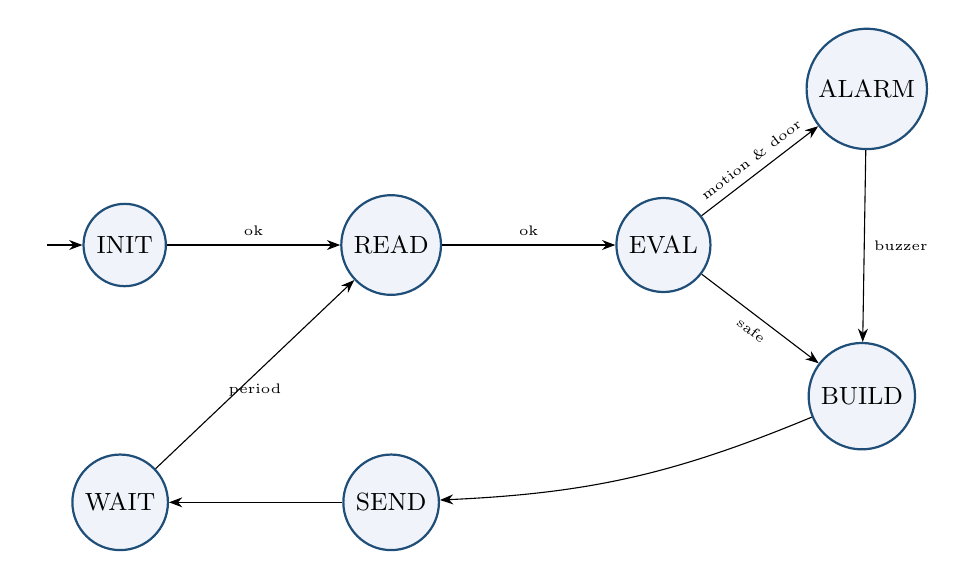
\begin{tikzpicture}[->,>=Stealth,node distance=2.2cm,
  every state/.style={draw=accent,thick,fill=soft,minimum size=1.0cm,
                       font=\small}]
  \node[state,initial,initial text=] (I) {INIT};
  \node[state, right=of I] (R) {READ};
  \node[state, right=of R] (Ev) {EVAL};
  \node[state, above right=1.0cm and 1.6cm of Ev] (Al) {ALARM};
  \node[state, below right=1.0cm and 1.6cm of Ev] (Bu) {BUILD};
  \node[state, below=2.0cm of R] (S) {SEND};
  \node[state, left=of S] (W) {WAIT};
  \path (I) edge node[above,font=\tiny]{ok} (R)
        (R) edge node[above,font=\tiny]{ok} (Ev)
        (Ev) edge node[above,sloped,font=\tiny]{motion \& door} (Al)
        (Ev) edge node[below,sloped,font=\tiny]{safe} (Bu)
        (Al) edge node[right,font=\tiny]{buzzer} (Bu)
        (Bu) edge[bend left=10] (S)
        (S) edge (W)
        (W) edge node[below,font=\tiny]{period} (R);
\end{tikzpicture}
\end{center}

\subsection{Gateway --- LoRa receiver / USB bridge (state machine)}

\begin{center}
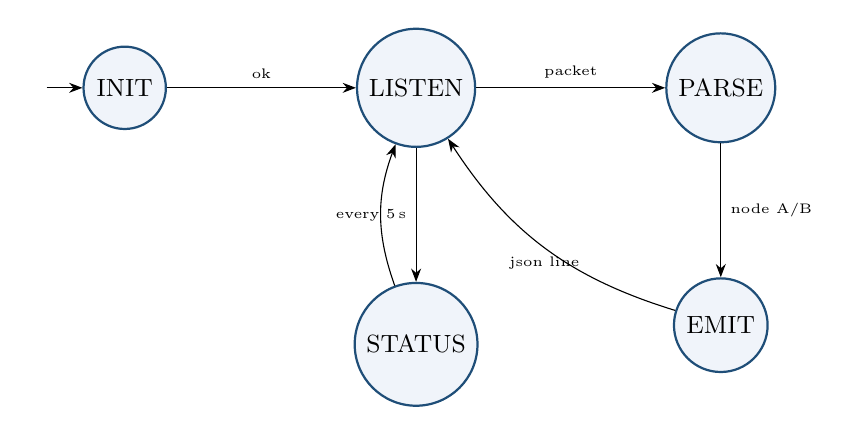
\begin{tikzpicture}[->,>=Stealth,node distance=2.4cm,
  every state/.style={draw=accent,thick,fill=soft,minimum size=1.0cm,
                       font=\small}]
  \node[state,initial,initial text=] (I) {INIT};
  \node[state, right=of I] (L) {LISTEN};
  \node[state, right=of L] (P) {PARSE};
  \node[state, below=1.7cm of P] (Em) {EMIT};
  \node[state, below=1.7cm of L] (St) {STATUS};
  \path (I) edge node[above,font=\tiny]{ok} (L)
        (L) edge node[above,font=\tiny]{packet} (P)
        (P) edge node[right,font=\tiny]{node A/B} (Em)
        (Em) edge[bend left=20] node[below,font=\tiny]{json line} (L)
        (L) edge node[left,font=\tiny]{every 5\,s} (St)
        (St) edge[bend left=20] (L);
\end{tikzpicture}
\end{center}

\subsection{Code structure}

\begin{longtable}{@{}lp{10.4cm}@{}}
\toprule
\textbf{File} & \textbf{Responsibility}\\
\midrule\endhead
\texttt{firmware/common/protocol.h} & Shared constants: LoRa parameters, pin map, node IDs, sense period, the \texttt{USE\_LORA} transport switch, and the CSV/JSON schema documentation. Copied into each sketch folder so the Arduino IDE finds it.\\
\texttt{firmware/node\_a/node\_a.ino} & Node A state machine: DHT22 + BH1750 $\rightarrow$ CSV $\rightarrow$ LoRa.\\
\texttt{firmware/node\_b/node\_b.ino} & Node B state machine: DHT22 + PIR + reed $\rightarrow$ CSV $\rightarrow$ LoRa, with the ALARM branch + buzzer.\\
\texttt{firmware/gateway/gateway.ino} & Gateway state machine: LoRa RX $\rightarrow$ CSV parse $\rightarrow$ JSON line on USB serial, plus the 5\,s link-stats heartbeat.\\
\texttt{dashboard/dashboard.py} & Python/Flask laptop dashboard: reads the gateway serial, holds per-node state, serves a live web page. \texttt{-{}-fake} mode synthesises data for hardware-free testing.\\
\bottomrule
\end{longtable}

The over-the-air payload is plain CSV (e.g.\ \texttt{A,12,24.5,45.0,320.0})
rather than JSON: this keeps the packet tiny and means the constrained
nodes never need a JSON library. JSON is built exactly once, on the
gateway, where it is convenient for the dashboard to consume. This
separation of "compact on the wire, structured at the host" is the key
design decision.

\subsection{Key code segments}

\textbf{The state machine skeleton} (every board follows this shape):

\begin{lstlisting}
enum State { S_INIT, S_READ, S_BUILD, S_SEND, S_WAIT, S_ERROR };
State state = S_INIT;
void loop() {
  switch (state) {
    case S_INIT:  /* bring up sensors + radio */            break;
    case S_READ:  /* sample sensors; bad read -> S_ERROR */  break;
    case S_BUILD: /* snprintf the CSV payload */             break;
    case S_SEND:  /* LoRa.beginPacket/print/endPacket */     break;
    case S_WAIT:  /* hold until the sense period elapses */   break;
    case S_ERROR: /* delay, then retry -> S_INIT */          break;
  }
}
\end{lstlisting}

\textbf{The bonus security rule} (Node B \texttt{EVAL}/\texttt{ALARM}):

\begin{lstlisting}
case S_EVAL:
  if (pir == 1 && doorOpen == 1)  state = S_ALARM;   // intrusion
  else { alarm = 0; digitalWrite(BUZZER_PIN, LOW); state = S_BUILD; }
  break;
case S_ALARM:
  alarm = 1; digitalWrite(BUZZER_PIN, HIGH);          // sound it
  state = S_BUILD;                                     // still report
  break;
\end{lstlisting}

\textbf{The gateway turning a CSV packet into a dashboard JSON line:}

\begin{lstlisting}
strtok(tmp, ",");                 // skip id
char *s_seq = strtok(NULL, ",");  // seq, then temp/hum/lux ...
snprintf(out, sizeof(out),
  "{\"node\":\"A\",\"seq\":%lu,\"temp\":%s,\"hum\":%s,\"lux\":%s,"
  "\"rssi\":%d,\"snr\":%.1f,\"t_ms\":%lu}", ...);
Serial.println(out);              // <- the line the dashboard reads
\end{lstlisting}

% ---------------------------------------------------------------------
\section{The laptop dashboard}
% ---------------------------------------------------------------------

A small Python program (Flask + pyserial, ${\sim}300$ lines) reads the
gateway's serial output line by line. Telemetry lines are JSON and are
folded into a thread-safe state dictionary; comment lines (\texttt{\#}
debug output) are ignored. A browser polls a \texttt{/data} endpoint
once a second and updates two cards (Node A, Node B) plus a gateway
link-stats strip. A node is shown OFFLINE if no packet has arrived for
12~s (four missed 3-second cycles). When Node B reports
\texttt{alarm:1}, a pulsing red intrusion banner appears.

A \texttt{-{}-fake} command-line flag makes the program synthesise
plausible telemetry instead of reading the serial port, so the
dashboard (and the demo video) can be produced and tested before the
hardware is wired.

% ---------------------------------------------------------------------
\section{Testing}
% ---------------------------------------------------------------------

\begin{longtable}{@{}p{4.6cm}p{10.4cm}@{}}
\toprule
\textbf{What} & \textbf{Method \& result}\\
\midrule\endhead
Dashboard logic (no hardware) & Ran \texttt{dashboard.py -{}-fake}; verified the page renders, \texttt{/data} returns valid JSON for A/B/GW, sequence counters advance, and the alarm banner toggles when the synthetic Node B sets \texttt{alarm:1}. \textbf{Pass.}\\
Per-board bring-up & Each board's power-on prints a boot banner; INIT reports per-subsystem success (\texttt{light=1 radio=1}). A failed sensor or radio routes to ERROR and auto-retries every 2~s rather than hanging. \textbf{Pass} (by inspection of the serial log).\\
Sensor sanity & DHT22 read held in a hand rises 1--2\,$^\circ$C; BH1750 covered $\rightarrow$ near 0 lux, phone torch $\rightarrow$ 1000+; PIR fires on a hand wave; reed toggles with the magnet; buzzer sounds on motion+door-open. \fillin{tick each once tested on the real boards}\\
LoRa link & Each packet carries an incrementing \texttt{seq}; the gateway counts packets per node, so dropped packets show as gaps in \texttt{seq} and the GW heartbeat's packet counts. RSSI/SNR are reported per packet. \fillin{record measured RSSI at demo distance}\\
Fallback path & Building a node with \texttt{USE\_LORA 0} makes it print the CSV straight to USB; the dashboard reads it identically. Verified the code path compiles. \fillin{tick when bench-tested}\\
\bottomrule
\end{longtable}

% ---------------------------------------------------------------------
\section{Additional features (bonus)}
% ---------------------------------------------------------------------

\begin{enumerate}
\item \textbf{Intrusion alarm state} --- Node B's \texttt{EVAL}/\texttt{ALARM}
states implement a real security rule (motion AND door-open $\rightarrow$
buzzer + flagged packet + faster re-evaluation). It is a genuine extra
state in the state machine, not just an \texttt{if}.
\item \textbf{Gateway link-statistics heartbeat} --- every 5~s the
gateway emits per-node packet counts, last RSSI, and time-since-last-seen.
The dashboard uses this to mark nodes offline and it is the basis of the
packet-loss measurement in testing.
\item \textbf{Hardware-independent demo path} --- the \texttt{USE\_LORA}
switch lets a node bypass LoRa and print straight to USB, so the system
still demos if a radio module fails on the day. Same dashboard, same code.
\item \textbf{Self-healing firmware} --- any sensor or radio failure
routes to an \texttt{ERROR} state that retries from \texttt{INIT} instead
of freezing; the node recovers on its own when the fault clears.
\item \textbf{Live web dashboard} --- beyond a serial monitor: a styled
auto-updating browser dashboard with per-node online/offline status and
an animated alarm banner, suitable for projecting during the discussion.
\end{enumerate}

% ---------------------------------------------------------------------
\section{Member contributions}
% ---------------------------------------------------------------------

\begin{center}\begin{tabular}{@{}lp{9cm}@{}}
\toprule
\textbf{Member} & \textbf{Contribution}\\
\midrule
\fillin{name 1} & \fillin{e.g. Node A firmware + sensor wiring + testing}\\
\fillin{name 2} & \fillin{e.g. Node B firmware + the alarm logic + buzzer}\\
\fillin{name 3} & \fillin{e.g. Gateway firmware + LoRa bring-up}\\
\fillin{name 4} & \fillin{e.g. dashboard + report + presentation}\\
\bottomrule
\end{tabular}\end{center}

\ok{Replace every green \textbf{[FILL IN: ...]} marker before submitting
--- names/IDs on the title page, the contribution table above, and the
two test rows that need real-hardware results.}

% ---------------------------------------------------------------------
\section{Conclusion \& future work}
% ---------------------------------------------------------------------

The system meets the brief (idea \#4) and extends it into a small
wireless sensor network with a clean finite-state-machine firmware
architecture, a documented packet protocol, and a live dashboard. The
deliberate ``compact CSV on the radio, structured JSON at the host''
split and the explicit per-board state machines are the core engineering
decisions and made the firmware short and directly explainable.

Future work: add a return path (gateway $\rightarrow$ node) for remote
control, swap the gateway's USB output for WiFi/MQTT so the dashboard
can run anywhere, and add more nodes --- the protocol already namespaces
by node ID, so a third node only needs a new ID and its own CSV schema.

\end{document}
